\documentclass[12pt,a4paper,openany]{book}
\usepackage{lmodern}
\usepackage[table]{xcolor}
\input{/home/aroquemaurel/cours/includesLaTeX/couleurs.tex}

\usepackage[utf8]{inputenc} \usepackage[T1]{fontenc}
\usepackage[francais]{babel}
\usepackage[top=1.7cm, bottom=1.7cm, left=1.7cm, right=1.7cm]{geometry}
\usepackage{verbatim}
\usepackage[urlbordercolor={1 1 1}, linkbordercolor={1 1 1}, linkcolor=vert1, urlcolor=bleu, colorlinks=true]{hyperref}
\usepackage{tikz} %Vectoriel
\usepackage{listings}
\usepackage{fancyhdr}
\usepackage{multido}
\usepackage{float}
\usepackage{amssymb}
\usepackage{longtable}
\usepackage{wrapfig}

\newcommand{\titre}{Conception d'une application Web -- SuperVod}

\newcommand{\pole}{}
\newcommand{\sigle}{bdd}

\newcommand{\semestre}{4}

\input{/home/aroquemaurel/cours/includesLaTeX/listings.tex}
\date{\today}

\makeindex
\lfoot{Université Toulouse III -- Paul Sabatier}
\rfoot{}
%\rfoot{}
\cfoot{}
\makeglossary
\makeatletter
\def\clap#1{\hbox to 0pt{\hss #1\hss}}%
\def\ligne#1{%
\hbox to \hsize{%
\vbox{\centering #1}}}%
\def\haut#1#2#3{%
\hbox to \hsize{%
\rlap{\vtop{\raggedright #1}}%
\hss
\clap{\vtop{\centering #2}}%
\hss
\llap{\vtop{\raggedleft #3}}}}%
\def\bas#1#2#3{%
\hbox to \hsize{%
\rlap{\vbox{\raggedright #1}}%
\hss \clap{\vbox{\centering #2}}%
\hss
\llap{\vbox{\raggedleft #3}}}}%
\def\maketitle{%
\thispagestyle{empty}\vbox to \vsize{%
\haut{}{\@blurb}{}

\vfill
\vspace{1cm}
\begin{flushleft}
\usefont{OT1}{ptm}{m}{n}
\huge \@title
\end{flushleft}
\par
\hrule height 4pt
\par
\begin{flushright}
\usefont{OT1}{phv}{m}{n}
\Large \@author
\par
\end{flushright}
\vspace{1cm}
\vfill
\vfill
\bas{}{\@location, le \@date}{}
}%
\cleardoublepage
}
\def\date#1{\def\@date{#1}}
\def\author#1{\def\@author{#1}}
\def\title#1{\def\@title{#1}}
\def\location#1{\def\@location{#1}}
\def\blurb#1{\def\@blurb{#1}}
\date{\today}
\author{}
\title{}
\location{Amiens}\blurb{}
\makeatother
\title{\titre}
\author{Base de données}

\location{Toulouse}
\blurb{%
Université Toulouse III -- Paul sabatier\\
L2 Informatique\\
\vspace{30px}
\begin{flushleft}Antoine de \bsc{Roquemaurel} (antoine.de-roquemaurel@univ-tlse3.fr)\\ 
	Fabrice \bsc{Valleix} (valleix.fabrice@gmail.com)\\
 Groupe 2.2\end{flushleft}
}%



%\title{Cours \\ \titre}
%\date{\today\\ Semestre \semestre}

%\lhead{Cours: \titre}
%\chead{}
%\rhead{\thepage}

%\lfoot{Université Paul Sabatier Toulouse III}
%\cfoot{\thepage}
%\rfoot{\sigle\semestre}

\pagestyle{fancy}
\renewcommand{\chaptermark}[1]{\markboth{\bsc{\chaptername~\thechapter{} :} #1}{}}
\renewcommand{\sectionmark}[1]{\markright{\thesection{ #1}}}
\renewcommand{\headrulewidth}{0.3pt}
\renewcommand{\footrulewidth}{0.3pt}

\fancyhf{}
\fancyhead[LE]{\leftmark}
\fancyhead[RO]{\rightmark}
\fancyfoot[LE,RO]{--~\thepage~--}
\fancyfoot[LO]{\titre{}}
\fancyfoot[RE]{Antoine de \bsc{Roquemaurel} -- Fabrice \bsc{Valleix}}

%% Cas des premières pages de chapitre
\fancypagestyle{plain}{%
	\fancyhf{}%
	\fancyfoot[L]{\titre{}}
	\fancyfoot[R]{--~\thepage~--}
	\renewcommand{\headrulewidth}{0pt}
	\renewcommand{\footrulewidth}{0.3pt}
}
\makeatletter
\renewcommand*{\lstlistlistingname}{Liste des codes sources}
\renewcommand\listoffigures{%
    \chapter{\listfigurename}%
      \@mkboth{\MakeUppercase\listfigurename}%
              {\MakeUppercase\listfigurename}%
       \@starttoc{lof}%
    }
    \renewcommand\listoftables{%
    \chapter{\listtablename}%
    \@mkboth{\MakeUppercase{\listtablename}}%
            {\MakeUppercase{\listtablename}}%
    \@starttoc{lot}
    }

    \renewcommand\lstlistoflistings{%
    \begingroup
    \chapter{\lstlistlistingname}%
    \parskip\z@\parindent\z@\parfillskip \z@ \@plus 1fil%
    \@starttoc{lol}%
    \endgroup
    }
	\makeatother

\input{/home/aroquemaurel/cours/includesLaTeX/remarquesExempleAttention.tex}
\input{/home/aroquemaurel/cours/includesLaTeX/polices.tex}
\input{/home/aroquemaurel/cours/includesLaTeX/affichageChapitre.tex}
\let\pagebreakORIG\pagebreak
\let\clearpageORIG\clearpage
\let\cleardoublepageORIG\cleardoublepage

\ifx \removepagebreak \undefined
\newcommand{\removepagebreak}{\renewcommand{\pagebreak}{}\renewcommand{\clearpage}{}\renewcommand{\cleardoublepage}{}}
\fi

\ifx \restorepagebreak \undefined
\newcommand{\restorepagebreak}{\renewcommand{\pagebreak}{\pagebreakORIG}\renewcommand{\clearpage}{\clearpageORIG}\renewcommand{\cleardoublepage}{\cleardoublepageORIG}}
\fi
\newcommand{\pfp}{\texttt{pfp}}

\newcommand{\ifp}{\texttt{if}}
\newcommand{\elsep}{\texttt{else}}

\makeatother
\includeonly {
}
\newcommand{\bootstrap}{\textit{bootstrap}}
\begin{document}
	\setcounter{tocdepth}{2}
	\setcounter{secnumdepth}{3}
	\removepagebreak
	\maketitle
	\newpage
	\chapter*{Avant-propos}
	Ce dossier comporte les différentes de réalisation de l'application Web SuperVod, site permettant de répertorier des séries.

	Il à été conçut par Antoine de \bsc{Roquemaurel} et Fabrice \bsc{Valleix} dans le cadre du module \textit{Systèmes d'Information et Application Web} de la L2 Informatique de l'université Toulouse III -- Paul Sabatier.

	\section*{Tester le projet}
	L'archive que vous avez reçus était organisée comme ceci: 
	\begin{description}
		\item[scriptCreationBd.sql] Contient le script de création de la base de données, le schéma n'a pas été changé, cependant \texttt{MySQL} étant sensible à la
			casse, des erreurs avait lieu avec le script de création qui nous étais fournis, ainsi par convention, toutes nos tables sont en minuscule.
		\item[superVod/] Contient tous les fichiers du Site Web. 
		\item[rapport.pdf] Le présent rapport que vous êtes en train de lire
	\end{description}

	Afin de tester le projet, vous pouvez avoir accès au site web fonctionnel directement en ligne à l'adresse \url{http://dev.joohoo.fr/dev/superVod/}. 
	Il est également possible d'utiliser notre code source avec votre propre serveur web et votre base de données, pour cela les paramétrage des accès à la base de données 
	sont présent dans le fichier \texttt{superVod/database/connect.php}. Toutes les adresses web étant en relatifs, aucun problème ne devrait avoir lieu.

	Ce site Web utilisant des fonctionnalités de \bsc{HTML}5 et \bsc{CSS}3, il est recommandé d'utiliser un navigateur récent. Ce site à été développé sous
	Google Chrome, ainsi l'affichage sera optimal sur ce navigateur, cependant il devrait s'afficher correctement sur les autres.

	Le site disposant d'un système d'upload d'image, afin que celui-ci fonctionne correctement, il est nécessaire que le dossier \texttt{images} possèdent les
	droits d'écritures pour le site web, soit les droits 777 dans le système Unix, ou appartenir au groupe \texttt{www-data}.

	Pour se connecter à la partie administration, les identifiants sont:
	\begin{description}
		\item[Login] admin
		\item[Mot de passe] admin
	\end{description}
	\vfill
	\footnotesize Rédigé le \today{} par Antoine de \bsc{Roquemaurel} et Fabrice \bsc{Valleix}
	\restorepagebreak
	\tableofcontents
	\chapter{Les besoins de l'application}
	Ce projet consiste en la création d'un site web utilisant les technologies \bsc{HTML}, \bsc{CSS}, \bsc{PHP} et la base de données \bsc{MySQL} permettant
	de répertorier des séries et leurs épisodes associés.  

	Pour cela le schéma de la base de données et un jeu d'essai nous à été fournis afin de pouvoir commencer rapidement le développement du site.
	\section{Affichage des séries et épisodes}
	La possibilité d'afficher dynamiquement les séries et leurs épisodes avec ainsi pour chaque série son titre, son nombre de saison et son nombre
	d'épisodes ainsi que son type, pour chaque épisode d'une série  son titre, sa saison, son numéro d'épisode son année de production, son réalisateur sa
	durée  et sa limite d'âge.

	Étant donné que le site est voué à disposé d énormément de séries différentes, plutôt que de tout afficher sur une page, nous avons souhaités ajouter un
	menu permettant de sélectionner la série. Cf image ?? page ??. % TODO screen accueil
	\section{Recherche de séries et épisodes}
	Le site doit permet d'effectuer des recherches, d'une part des recherches d'épisodes, en fonction d'une partie du titre, ses année de production, son type,
	son age minimum, toutes les séries trouvés grâce à la recherche permette d'afficher les épisodes de la série.

	Mais il doit également être possible de chercher un épisode en fonction de la série concernée, de son année de diffusion, de sa saison et de ses différents
	prix d'achats maximum (Streaming, location ou achat) dans le cas où on souhaite acheter un épisode.

	Des captures d'écrans de recherches sont disponibles image ?? et ?? page ??. % TODO screen recherche
	\section{Ajout de série et épisode}
		Afin que le dynamisme du site ai un intérêt, il devait être possible d'ajouter des séries ou des épisodes dynamiquement. Ainsi une partie administration
		à été créé afin que seul l'administrateur puisse ajouter des séries. Lors de l'ajout d'une série ou d'un épisode, une image peut être téléchargée sur le
		site à l'aide d'un formulaire d'envoi.

	\chapter{Organisation du travail d'équipe}
	Pour ce projet, nous étions deux à travailler dessus, ainsi nous avons utilisé plusieurs techniques afin de se coordonner et de limiter les problèmes. Ceci
	n'est pas notre premier projet ensemble, notre travail en fut simplifié.
	\section{Un outil de gestion de projet : Redmine}
	\begin{figure}[H]
		\centering
		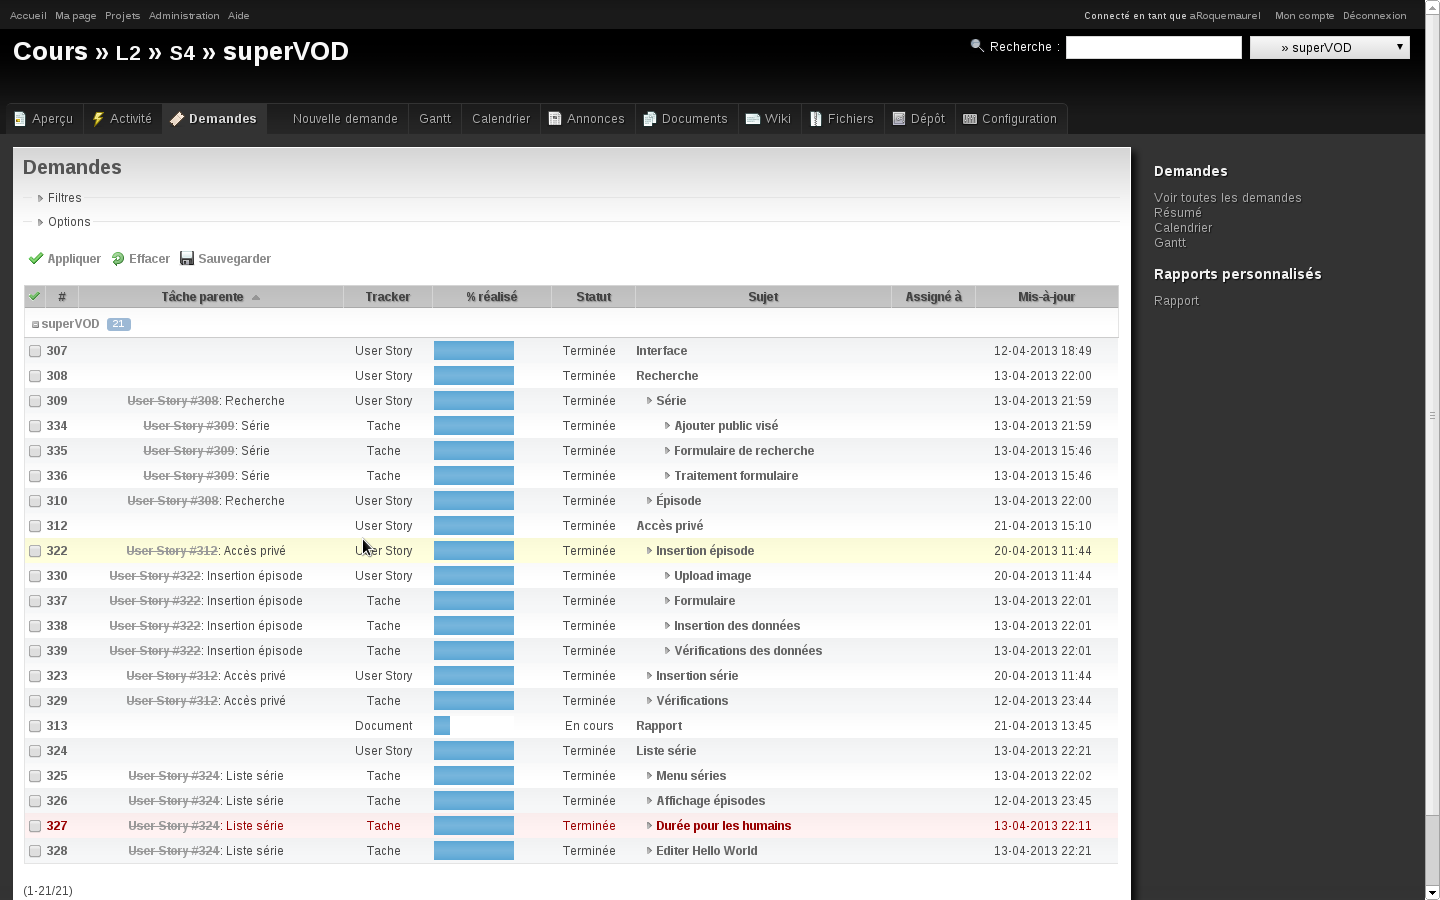
\includegraphics[width=18cm]{screens/redmine.png}
		\caption{Affichage des demandes dans Redmine}
		\label{fig:redmine}
	\end{figure}
	Pour le projet, nous avons utiliser \textit{Redmine}, une plateforme web de gestion de projet (Cf figure \ref{fig:redmine}). Elle nous a permis de simplifier le travail, et
	de ne rien oublier.

	En effet, nous pouvons créer des tâches, signaler qu'elles sont en cours/terminés/en tests, leur donner des dates limites, les affecter à une personne etc\ldots
	Ainsi lorsque l'un de nous commençait une tâche, il le signalait sur le \textit{redmine}, ce qui permettait de tenir au courant son binôme de ses actions et
	de l'avancée du projet.

	\section{Un logiciel de versionnement : Git}
	Afin de limiter les problèmes du travail collaboratif, nous avons utilisé un logiciel de versionnement Git. Il a deux intérêt, tout d'abord, nous pouvons
	travailler à deux en parallèle sur le projet sans se soucier de fusionner notre travail\footnote{À condition de ne pas travailler sur deux lignes de code
	identiques}.

	D'autre part, tous les logs étant enregistrés, nous pouvons savoir qui à fait quoi et quel jour, cela permet de voir également l'avancée du projet. 

	Enfin, toutes les modification sont stockées sur le serveur, ainsi en cas de problème, il est très facile de revenir à la version précédente ou même de
	comparer deux versions afin de voir les changements et de comprendre rapidement pourquoi une fonctionnalité à régressé. 

	\section{Répartition des tâches}
	Nous nous sommes répartis les tâches afin de travailler efficacement, en fonction de nos domaines d'affinités et d'expertise, ainsi Fabrice s'occupait
	plutôt de la partie base de données et \bsc{SQL} pendant qu'Antoine architecturait l'application afin qu'elle soit la plus cohérente possible, le reste du projet
	était fait sans répartition particulière, en fonction des besoins et de l'envie de chacun.

	\chapter{Implémentation et conception}
		La conception du projet est l'étape la plus importante, ainsi nous avons préférés repenser à notre manière le projet, 
		nous sommes partis sur une architecture respectant plus le patron de conception MVC\footnote{Modèles Vue Contrôleur ou
		\textit{pattern MVC} : Model View Controller en anglais}, c'est à
		dire que toute la partie affichage (notamment le \bsc{HTML}), Modèle (c'est-à-dire les requêtes \bsc{SQL}) sont séparés, c'est le Contrôleur qui dirige le
		modèle et la vue, c'est ainsi le \textit{chef d'orchestre}.
		\section{Mise en forme : les vues}
			Afin d'avoir un site web élégant sans passer beaucoup de temps à réinventer la roue en \bsc{CSS}, nous avons choisis d'utiliser un
			framework\footnote{Kit de composants logiciels structurels, qui sert à créer les fondations ainsi que les grandes lignes de tout ou d’une partie d'un
			logiciel (architecture). --- D'après \textit{wikipédia}} CSS
			appelé \bootstrap{}. Celui-ci nous permet d'avoir une mise en forme sobre très rapidement.  La mise en forme est organisé comme suit:

			\subsection{Le CSS} Le \bsc{css} est présent dans le dossier \texttt{style/css}, dedans nous avons d'une part le \bsc{css} fourni par \bootstrap{}, auquel nous
			n'avons pas touché, d'autre part, notre \bsc{css} qui surcharge certains affichage de \bootstrap{}, celui-ci est dans \texttt{style/css/style.css}.
			\lstinputlisting[language=CSS, caption=Exemple d'une partie du CSS]{code/css.css}
				
			\subsection{Le JavaScript}
			Les bibliothèques JavaScript utilisées par \textit{\bootstrap{}} sont présentes dans \texttt{style/js}, celle-ci nous n'y avons
					pas touchés, le code JavaScript que nous avons développé étaient toujours très simple, ceci dût au travail de \bootstrap{}, ainsi il est présent
					en fin de page \bsc{HTML} le cas échéant.
			\lstinputlisting[language=javascript, mathescape=false, caption=Code javascript grisant le champ de prix lors de l'ajout d'un épisode]{code/js.js}
		\subsection{Le \bsc{HTML}}
		Le \bsc{html} correspond aux vues, tous nos fichiers contenant du HTML sont dans le dossier \texttt{views/}, les formulaires 
		eux sont dans le dossier \texttt{views/forms}.
		
		Les vues peuvent ne comporter que du \bsc{html}, comme c'est le cas dans les formulaires, mais ils peuvent également comporter des instructions simples
		de \bsc{php} comme des boucles ou des conditions.

		Le dossier \texttt{views} contient également les fonctions de série et épisode servant uniquement à l'affichage de ceux-ci.
			\lstinputlisting[language=PHP, mathescape=false, caption=Vue de la page permettant de rechercher une série]{code/vue.php}
		\section{Connexions à la base de données : Les modèles}
		L'application ne comporte que deux modèles : un pour les séries et un pour les épisodes, ces deux fichiers contiennent des fonctions effectuant des
		requêtes et retournant un tableau avec les attributs, ceci afin de bien séparer le \bsc{sql} du \bsc{php}.

		Également présent dans le dossier \texttt{database}, le fichier \texttt{connect.php} contient les identifiants et les instructions de connexion à la base de données.

		\lstinputlisting[language=SQL, mathescape=false, caption=Requête sélectionnant toutes les séries]{code/sql.sql}
		\lstinputlisting[language=PHP, mathescape=false, caption=Requête recherchant des épisodes]{code/sql.php}
		\section{Liaison des vues aux modèles : Les contrôleurs}
		Chaque contrôleur correspond aux pages que verra un utilisateur lambda dans l'URL, les contrôleurs sont en général assez simples, ils font appels au
		modèle puis font une inclusion de la vue, ceux sont eux qui feront les éventuels vérifications sur des paramètres, sur une connexion pour la partie
		privée etc\ldots
		\lstinputlisting[language=PHP, mathescape=false, caption=Contrôleur de la page d'accueil]{code/controleur.php}
		Comme dit plus haut, c'est relativement simple, on inclus les vues et fonctions nécessaires, on demande l'obtention des séries, on fait quelques
		vérifications puis on affiche la vue de la page d'accueil.
	\chapter{Résultats obtenus}
	Dans cette partie, nous allons regrouper quelques captures d'écrans montrant les résultats obtenus sur notre application Web. L'application est répartie en 3
	fonctionnalités : 
	\begin{itemize}
		\item L'affichage des séries et épisodes présents
		\item La recherche de série ou épisodes
		\item L'ajout de série ou épisodes
	\end{itemize}
	L'ajout d'épisodes implique la possibilité de se connecter afin que seul l'administrateur puisse utiliser l'administration.
	\remarque{Le couple login/mot de passe de l'application est admin/admin}
	\section{Affichage des séries et épisodes}
	\begin{figure}[H]
		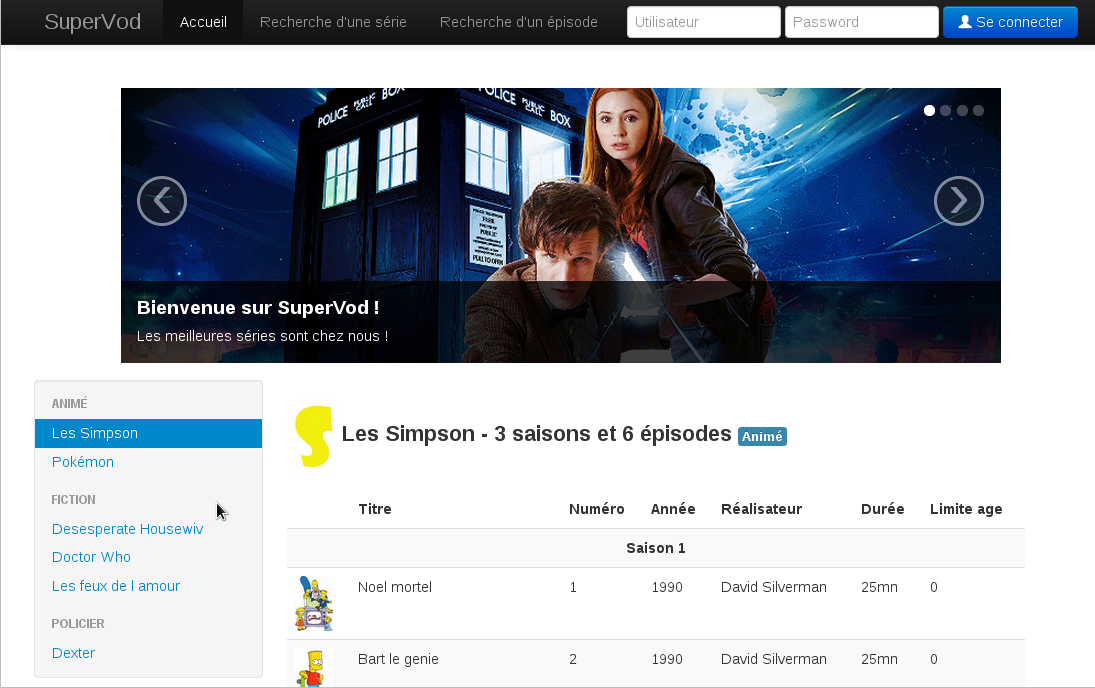
\includegraphics[width=18.0cm]{screens/accueil.png}
		\caption{Page d'accueil de l'application}
		\label{fig:accueil}
	\end{figure}
	La figure \ref{fig:accueil} nous montre la page d'accueil du site, avec la possibilité de sélectionner une série via le menu de gauche, affichant ainsi tous
	ses épisodes. On peut remarquer sur cette figure que le site possède un thème qui est commun à tout le site : la barre de navigation en haut de l'écran
	permet d'accéder d'un clique à chacune des fonctionnalités présentes sur le site.
	\section{Recherche}
	\begin{figure}[H]
		\centering
		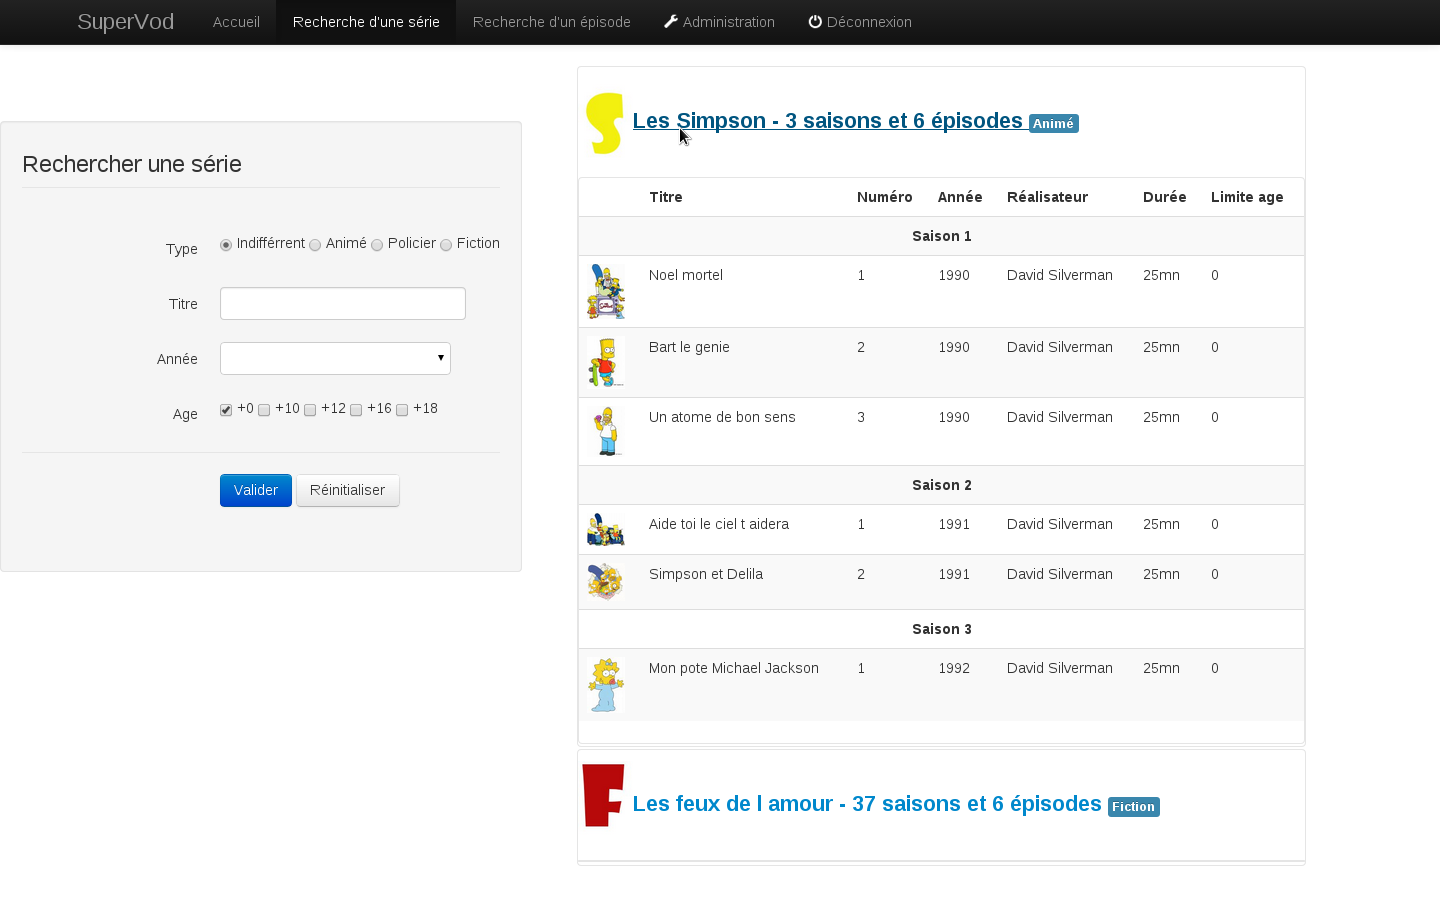
\includegraphics[width=15.7cm]{screens/rechercheSerie.png}
		\caption{Recherche d'une série}
		\label{fig:rechercheSerie}
	\end{figure}
	\begin{figure}[H]
		\centering
		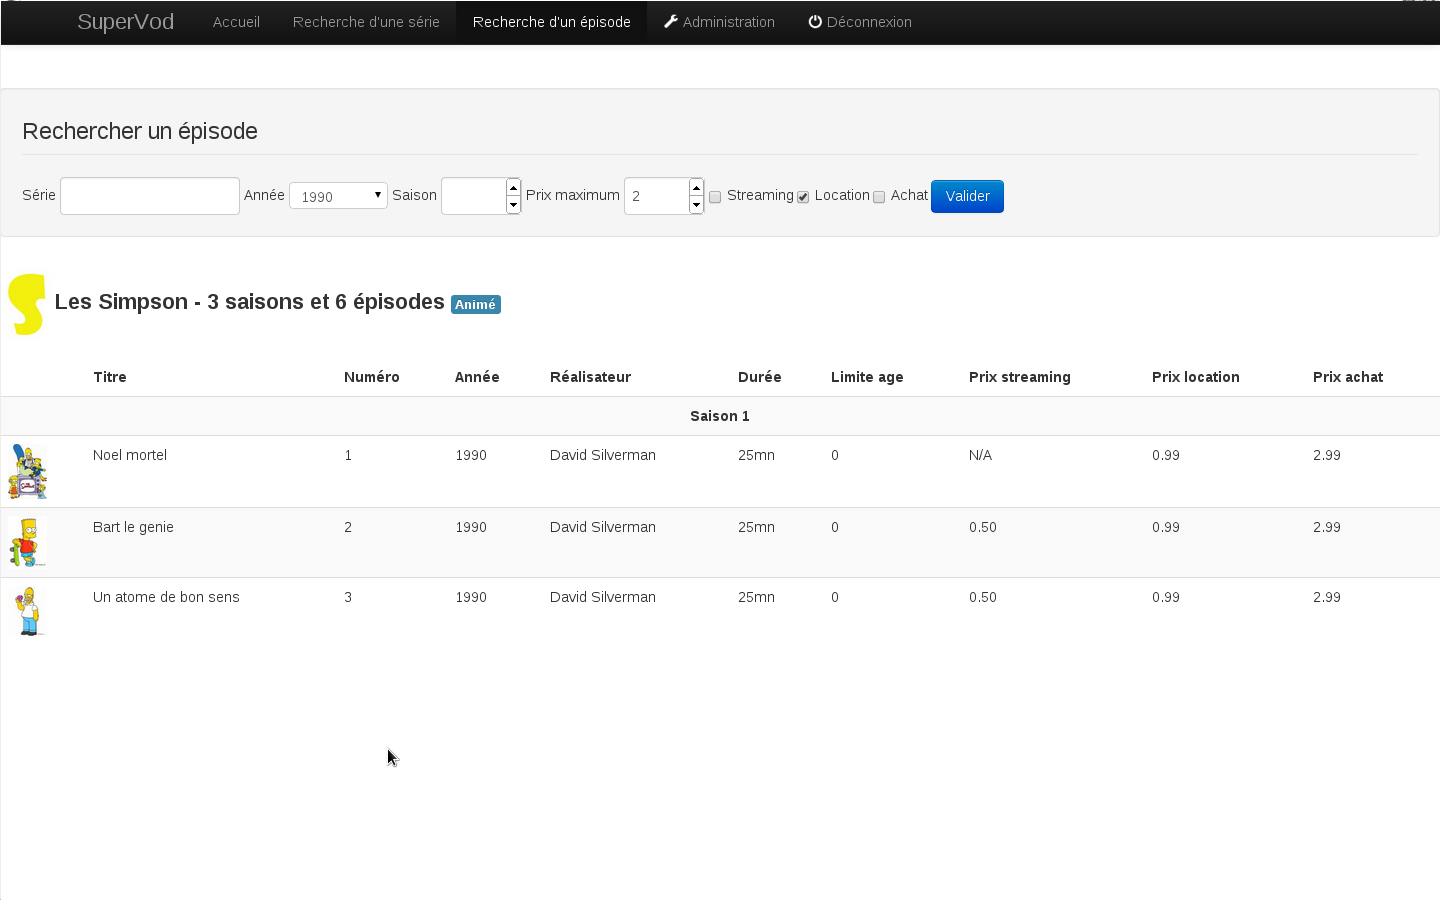
\includegraphics[width=15.7cm]{screens/rechercheEpisodes.png}
		\caption{Recherche d'un épisode}
		\label{fig:rechercheEpisode}
	\end{figure}
	Les figures \ref{fig:rechercheSerie} et \ref{fig:rechercheEpisode} nous montrent respectivement la recherche d'une série et la recherche d'un épisode.

	Ces deux fonctionnalités sont assez similaires, bien que les critères de recherches soit différents. Ainsi, la recherche d'une série affiche les séries
	répondants au critères renseignés\footnote{Une série peut être cherché par son type, son titre, ses années de diffusion ainsi que son age}, ainsi que la
	possibilité d'affiche les épisodes correspondants de la série.

	La recherche d'un épisode quand à elle à une mise en forme différente, étant donné qu'il y a plus d'informations a afficher pour un épisode, cependant le
	principe reste le même via les critères de recherche\footnote{Un épisode peut être trouvé grâce à sa série, son année de diffusion, sa saison, le prix
	maximum auquel on veut l'acheter, ainsi que sa disponibilité (Streaming, Location, Achat)}
	\section{Ajout de séries et épisodes}
	\begin{figure}[H]
		\centering
		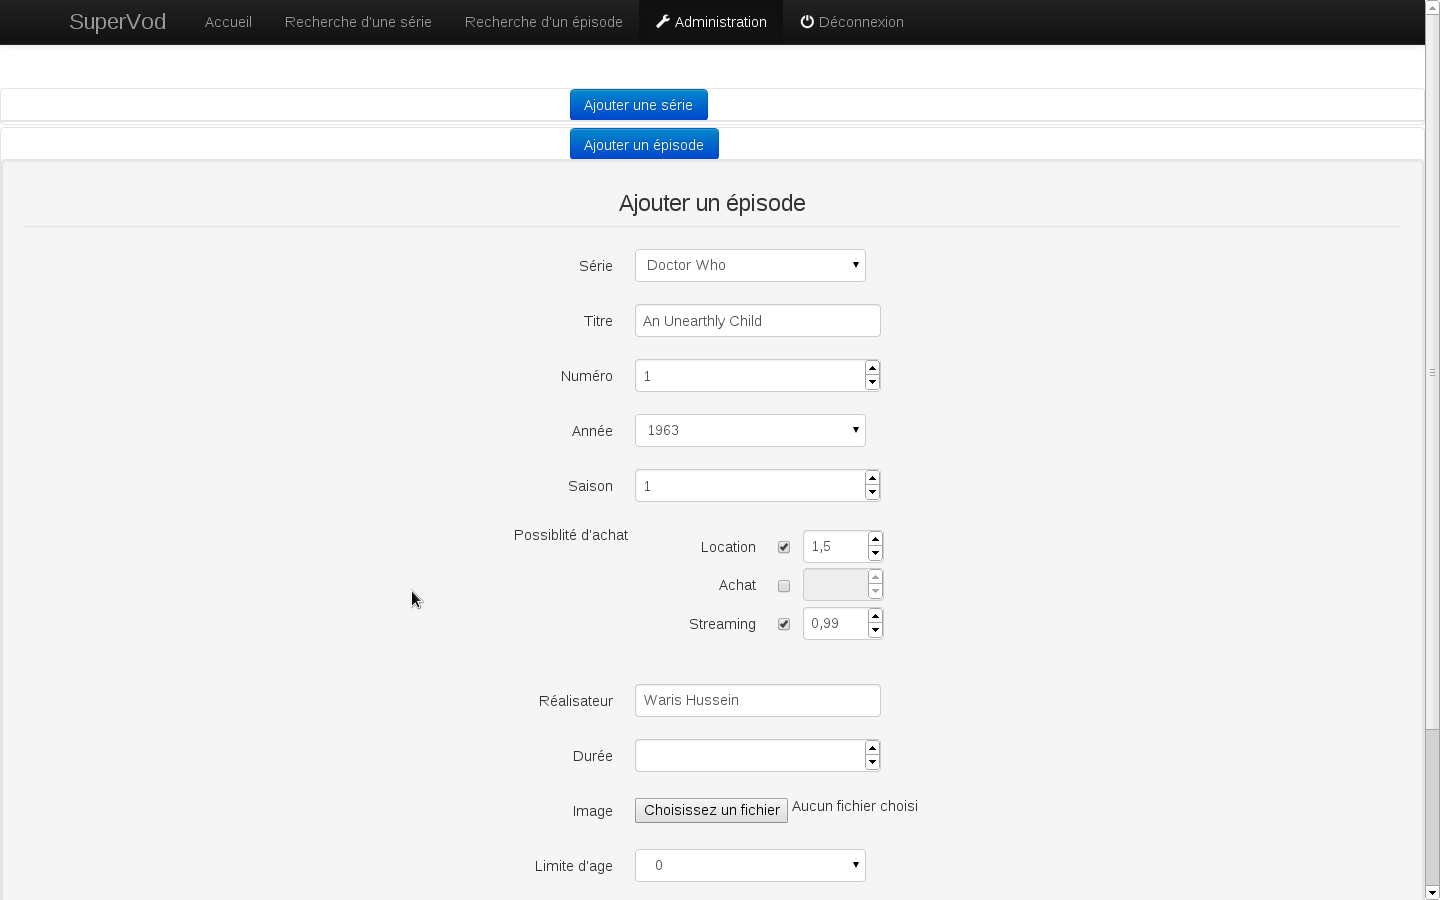
\includegraphics[width=18.5cm]{screens/adminEpisode.png}
		\caption{Administration}
		\label{fig:admin}
	\end{figure}
	La figure \ref{fig:admin} nous montre la partie administration, ici l'ajout d'un nouvel épisode à la série \textit{Doctor Who}, tous les champs présents
	précédemment peuvent être renseignés, cependant seuls les champs Série, Titre, Numéro et Saison sont obligatoires, les autres sont facultatifs.\\
	Il est également possible de sélectionner une image pour la série depuis notre ordinateur via un champ d'upload.

	Nous n'avons pas fait de capture d'écrans de l'ajout d'une série, cependant le principe est le même bien que les champs soient moins nombreux, pour une
	série, les champs Type et Nom sont obligatoires.
	\section{Valide HTML5}
	\begin{figure}[H]
		\centering
		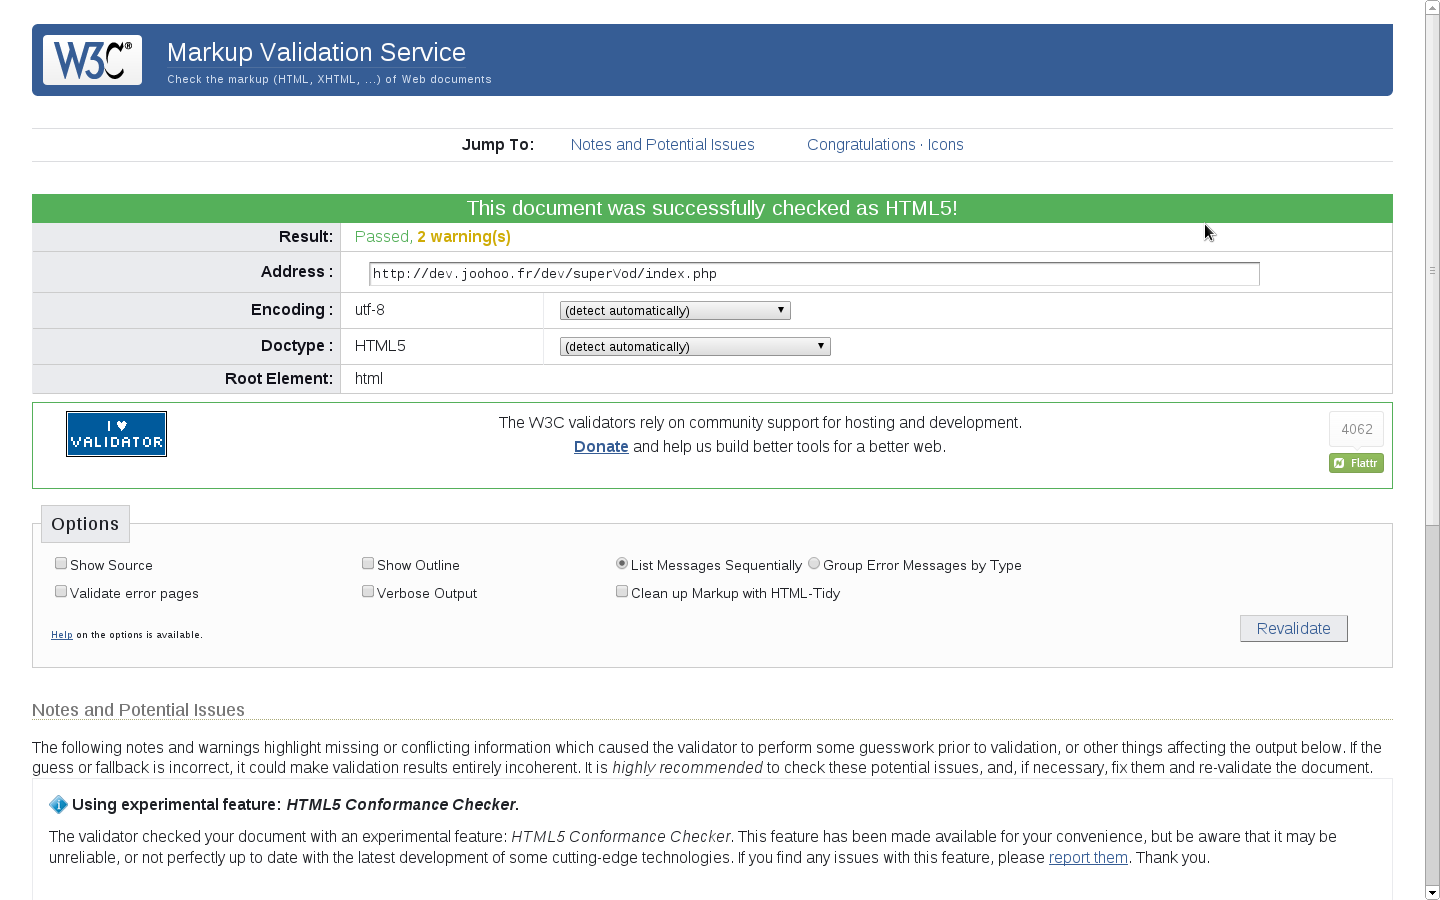
\includegraphics[width=17cm]{screens/htmlValidator.png}
		\caption{HTML5 validator -- Passed}
		\label{fig:htmlValidator}
	\end{figure}
	La figure \ref{fig:htmlValidator} montre simplement notre site web passant la validation du \bsc{w3c}\footnote{World Wide Web Consortium} avec la norme
	HTML5.
	\appendix
	\listoffigures
	\removepagebreak
	\vfill
	\lstlistoflistings
	\vfill
	\restorepagebreak
\end{document}

